%% LyX 2.1.2 created this file.  For more info, see http://www.lyx.org/.
%% Do not edit unless you really know what you are doing.
\documentclass[english,article]{jss}
\usepackage[T1]{fontenc}
\usepackage[latin9]{inputenc}
\usepackage{array}
\usepackage{float}
\usepackage{multirow}
\usepackage{amsbsy}
\usepackage{graphicx}
\usepackage[authoryear]{natbib}

\makeatletter

%%%%%%%%%%%%%%%%%%%%%%%%%%%%%% LyX specific LaTeX commands.
%% Because html converters don't know tabularnewline
\providecommand{\tabularnewline}{\\}
\floatstyle{ruled}
\newfloat{algorithm}{tbp}{loa}
\providecommand{\algorithmname}{Algorithm}
\floatname{algorithm}{\protect\algorithmname}

%%%%%%%%%%%%%%%%%%%%%%%%%%%%%% Textclass specific LaTeX commands.
 %\usepackage{Sweave}

%%%%%%%%%%%%%%%%%%%%%%%%%%%%%% User specified LaTeX commands.
%the following commands are used only for articles and codesnippets
\usepackage{amsmath}
\usepackage{amssymb}
\DeclareMathOperator*{\argmax}{arg\,max}
\DeclareMathOperator*{\argmin}{arg\,min}

\author{Zhaozhi Qian\\The University of Hong Kong \And 
       Philip L.H. Yu\\The University of Hong Kong}
\title{Weighted Distance-based Models for Ranking Data using the \proglang{R} Package \pkg{rankdist}}

% the same as above, without any formatting
\Plainauthor{Zhaozhi Qian,  Philip L.H. Yu}
\Plaintitle{Weighted Distance-based Models for Ranking Data using the R Package rankdist} 
%if necessary, provide a short title
\Shorttitle{Package \pkg{rankdist} in \proglang{R}} 

\Abstract{\pkg{rankdist} is a recently developed \proglang{R} package which implements various distance-based ranking models. These models capture the occurring probability of rankings based on the distances between them. The package provides a framework for fitting and evaluating finite mixture of distance-based models. This paper also presents a new probability model for ranking data based on a new notion of weighted Kendall distance. The new model is flexible and more interpretable than the existing models. We show that the new model has an analytic form of the probability mass function and the maximum likelihood estimates of the model parameters can be obtained efficiently even for ranking involving a large number of objects. In this paper, we also provide some examples on the usage of the package. The examples also demonstrate the advantage of the new model in different aspects.}
%at least one keyword is needed
\Keywords{Ranking data, Distance-based models, Kendall distance, Mixtures models, Rank aggregation, \proglang{R}}
%the same as above, without any formatting
\Plainkeywords{Ranking data, Distance-based models, Kendall distance, Mixtures models, Rank aggregation, R} 

%the following commands are used only for book or software reviews

%\Reviewer{Some Author\\University of Somewhere}
%\Plainreviewer{Some Author}

%the following commands are used only for book reviews
%\Booktitle{LyX and \proglang{R}: Secrets of the LyX Master}
%\Bookauthor{Book Author}
%\Pubyear{2008}
%\ISBN{0-12345-678-9}
%\Pages{500}

%the following command is used only for software reviews
%\Softwaretitle{\proglang{gretl 1.7.4}}

%the following commands are used only for book or software reviews
%\Publisher{LyX Publishing Inc.}
%\Pubaddress{LyX City}
%\Price{USD 59.95 (P), USD 99.95 (H)}
%\URL{http://www.lyx.org/}

%without any formatting
%\Plaintitle{LyX and R: Secrets of the LyX Master}
%\Shorttitle{LyX and R}

%the following commands are used for articles, codesnippets, book reviews and software reviews

%publication information
%do not use these commands before the article has been accepted
%\Volume{00}
%\Issue{0}
%\Month{Month}
%\Year{2000}
%\Submitdate{2000-00-00}
%\Acceptdate{2000-00-00}

%The address of at least one author should be given in the following format
\Address{
  Zhaozhi Qian\\
  The University of Hong Kong\\
  Hong Kong, China\\
  E-mail: \email{qianzhaozhi@connect.hku.hk}
}
\Address{
Zhaozhi Qian\\
  The University of Hong Kong\\
  Hong Kong, China\\
  E-mail: \email{qianzhaozhi@connect.hku.hk}\\
  Philip L.H. Yu\\
Department of Statistics and Actuarial Science\\
  The University of Hong Kong\\
  Hong Kong, China\\
  E-mail: \email{plhyu@hku.hk}
}
%you can add a telephone and fax number before the e-mail in the format
%Telephone: +12/3/4567-89
%Fax: +12/3/4567-89

%if you use Sweave,  include the following line (with % symbols):
%% need no \usepackage{Sweave.sty}

\makeatother

\usepackage{babel}
\begin{document}



\section[Introduction]{Introduction}

Ranking data occur when raters are asked to rank order a set of objects.
Examples of ranking data arise in elections, movie rankings, shopping
preferences and so on. By analyzing ranking data, we may want to understand
the patterns of rank-order preferences of raters and to find the most
representative ranking generally consented by the raters. Ranking
data analysis thus has important applications in market research,
recommendation systems and political sciences.

In a survey paper, \citet{Critchlow1986} broadly categorized probability
models for ranking data into four classes: (1) order statistics models,
(2) paired comparison models, (3) distance-based models, and (4) multistage
models. For more details, please refer to the monograph by \citet{AlvoYu2014}.
Among them, the order statistics models have the longest history.
Typical examples of these include independent order statistics models
\citep{Thurstone1927,Luce1959} and multivariate order statistics
models \citep{Yu2000,Joe2001}. The basic idea behind these models
is that each rater assigns a latent score or utility to each object
according to his/her perception of the object and the ordering of
these utility scores then determines the rater's ranking of the objects.
While this approach works well when the number of objects is small,
its parameter estimation often becomes computationally demanding when
a large number of objects are ranked. Both the paired comparison models
\citep{Smith1950,Mallows1957} and the multistage models \citep{Fligner1988}
try to decompose the ranking process into a set of independent decisions
where each decision can be to compare a pair of objects considered
in the decision or to count the number of ``mistakes'' generated
in the decision. A common critique of these two approaches is that
the assumed cognitive model of assigning rankings may not always be
true. Distance-based models \citep{Diaconis1988} rely on distance
metrics between two rankings. They were not as popular as the above
three models until recently because they were thought to be too inflexible.
This paper introduces the \proglang{R} package \pkg{rankdist} which
provides a unified way to fit different distance-based ranking models.
This paper also presents a original model which has an elegant analytic
form of the probability mass function.

The paper is organized as follows. In Section 2, we review the general
formulation of distance-based models and several well-known examples.
We then introduce the weighted Kendall distance and formulate the
weighted Kendall distance model in Section 3. Section 4 shows possible
ways to extend distance-based models. We give details on the package
architechture and implementation in Section 5. In Section 6, we illustrate
the usage of package \pkg{rankdist} with simulated examples. In Section
7, we present the results of applying different models to APA Election
data set using package \pkg{rankdist} and compare their performance
in terms of goodness of fit and interpretability. We also apply our
model to rank aggregation tasks, and compare the results to aggregated
ranking based on the Borda count. Finally, we discuss the strengths
of our new model and directions for future development of the \pkg{rankdist}
package.

Before we introduce the model in full details, it is helpful for us
to review some important conventions of permutation notations. In
the rest of this paper, permutations are denoted as lower-case Greek
letters $\pi,\sigma,\tau$ etc. $\pi(i)$ denotes the rank given to
object $i$, and $\pi^{-1}(i)$ denotes the object assigned the rank
$i$. The total number of objects in the ranking is $t.$ For any
two permutations $\pi$ and $\sigma$, the product $\tau=\pi\sigma$
is defined by the equation $\tau(i)=\pi(\sigma(i)),i=1,2,\cdots,t$. 


\section[Distance-based ranking models]{Distance-based ranking models}


\subsection[Overview]{Overview of distance-based models}

Sometimes it is reasonable to assume that there exists a modal ranking
$\pi_{0}$ which has the highest probability to occur and most observed
rankings are close to $\pi_{0}$. Thus we should assign the highest
probability to $\pi_{0}$ and for any other ranking the probability
should be negatively correlated with its distance from $\pi_{0}$.
According to this framework, \citet{Diaconis1988} proposed a family
of distance-based model,

\begin{equation}
\Prob(\pi|\lambda,\pi_{0})=\frac{e^{-\lambda D(\pi,\pi_{0})}}{C(\lambda)}\label{eq:dist_model_def}
\end{equation}
where $\pi_{0}$ denotes the modal ranking, $D(\pi,\pi_{0})$ is a
distance function between $\pi$ and $\pi_{0}$, $\lambda\geq0$ is
the dispersion parameter and $C(\lambda)$ is the normalization constant.
The usual properties of $D(\pi,\pi_{0})$ are: (1) reflexivity, $d(\pi,\pi)=0$;
(2) positivity, $d(\pi,\sigma)>0$ if $\pi\neq\sigma$; and (3) symmetry,
$d(\pi,\sigma)=d(\sigma,\pi)$. For ranking data, the distance should
also satisfy an additional property: (4) right-invariance, $d(\pi,\sigma)=d(\pi\nu,\sigma\nu)$
for any permutation $\pi,\sigma$ and $\nu$. This ensures that a
relabeling of the objects has no effect on the distance. If a distance
satisfies the triangular inequality: (5) $d(\pi,\nu)\leq d(\pi,\sigma)+d(\sigma,\nu)$,
the distance is said to be a metric. The commonly used distances include 
\begin{enumerate}
\item Kendall distance:
\[
D_{K}(\pi,\sigma)=\sum_{i<j}I\left\{ \left[\pi(i)-\pi(j)\right]\left[\sigma(i)-\sigma(j)\right]<0\right\} ,
\]
where $I\{\cdotp\}$ is the indicator function taking values 1 or
0 depending on whether the statement in brackets holds or not.
\item Spearman distance:
\[
D_{S}(\pi,\sigma)=\frac{1}{2}\sum_{i=1}^{t}\left[\pi(i)-\sigma(i)\right]^{2}
\]

\item Hamming distance:
\[
D_{H}(\pi,\sigma)=t-\sum_{i=1}^{t}\sum_{j=1}^{t}I\left\{ \pi(i)=j\right\} I\left\{ \sigma(i)=j\right\} 
\]

\item Footrule distance:
\[
D_{F}(\pi,\sigma)=\sum_{i=1}^{t}|\pi(i)-\sigma(i)|
\]

\item Cayley distance: $D_{C}$ is defined as the minimum number of transpositions
needed to transform one ranking into the other. 
\end{enumerate}
Note that the Spearman footrule and Kendall distances are metrics.
These distance measures are developed in different settings. For example
the Hamming distance is closely related to coding theory and the Cayley
distance has an intimate relationship with the Cayley graph in group
theory. Each of these distances can be formulated into a ranking model
as in (\ref{eq:dist_model_def}). However, these models do not generally
have a tractable normalization constant $C(\lambda)$, which limits
their practical use. 


\subsection[Mallows' phi model]{Mallows' $\phi$ model\label{sub:Mallows'--model}}

Among the above-mentioned distance functions, the Kendall disance
is the most popular one as its distance-based model, also called the
Mallows' $\phi$ model \citep{Mallows1957}, can have a closed-form
normalization constant:

\[
C(\mathbf{\lambda})=\prod_{i=1}^{t-1}\frac{1-e^{-(t-i+1)\lambda}}{1-e^{-\lambda}}.
\]
In addition, Kendall distance satisfies all five properties given
in the last section. It  can also be interpreted as the minimum
number of adjacent transpositions required to transform $\pi$ to
$\sigma$.

 Although the Mallows' $\phi$-model has a closed-form normalization
constant, it may be too restrictive since it has only one model parameter.
Efforts have been taken to introduce more flexibility into the Mallows'
$\phi$-model, and we will describe two such examples below. 


\subsection[Phi-component model]{The $\phi$-component model}

The $\phi$-component model proposed by \citet{Fligner1986} is a
generalization of Mallows' $\phi$-model. Its basic idea is motivated
by the fact that the Kendall distance can be decomposed into a sum
of $t-1$ scores $V_{i}(\pi,\sigma),i=1,,\cdots,t-1$ obtained in
a ranking process:
\[
D_{K}(\pi,\sigma)=\sum_{i=1}^{t-1}V_{i}(\pi,\sigma),
\]
where
\begin{equation}
V_{i}(\pi,\sigma)=\sum_{j=i+1}^{t}I\{[\pi(\sigma^{-1}(i))-\pi(\sigma^{-1}(j))]>0\}.\label{eq:1}
\end{equation}
Here $V_{1}(\pi,\sigma)$ represents the number of adjacent transpositions
needed to place the object $\sigma^{-1}(1)$ (the object ranked first
in $\sigma$) in the first position in ranking $\pi$. In the $i$th
stage ($2\le i\le t-1$), $\pi^{-1}(j)=\sigma^{-1}(j)$ for $j=1,\cdots,i-1$,
and $V_{i}(\pi,\sigma)$ is the number of adjacent transpositions
needed to place the object $\sigma^{-1}(i)$ in the $i$th position
in ranking $\pi.$ Therefore, the ranking can be described as $t-1$
stages where $V_{i}(\pi,\sigma)$ can be interpreted as the number
of mistakes made in assigning rank to object $\sigma^{-1}(i)$ after
$(i-1)$ stage and it takes value $0,1,\cdots,(t-i)$. 

The $\phi$-component model introduces dispersion parameter $\lambda_{i}$
for each $V_{i}(\pi,\pi_{0})$, and takes the form of:
\begin{equation}
\Prob(\pi|\mathbf{\boldsymbol{\lambda}},\pi_{0})=\frac{e^{-\sum_{i=1}^{t-1}\lambda_{i}V_{i}(\pi,\pi_{0})}}{C(\mathbf{\boldsymbol{\lambda}})},\label{eq:phi_component}
\end{equation}
where $\boldsymbol{\mathbf{\lambda}}=(\lambda_{1},\cdots,\lambda_{t-1})'$
and $C(\boldsymbol{\mathbf{\lambda}})$ is the normalization constant,
which equals

\[
C(\mathbf{\boldsymbol{\lambda}})=\prod_{i=1}^{t-1}\frac{1-e^{-(t-i+1)\lambda_{i}}}{1-e^{-\lambda_{i}}}\equiv\prod_{i=1}^{t-1}C(\lambda_{i}).
\]
Thus (\ref{eq:phi_component}) can be simplified as

\begin{equation}
\Prob(\pi|\mathbf{\boldsymbol{\lambda}},\pi_{0})=\prod_{i=1}^{t-1}\frac{e^{-\lambda_{i}V_{i}(\pi,\pi_{0})}}{C(\lambda_{i})}\label{eq:phi_component_simp}
\end{equation}
which is a joint probability mass function of $t-1$ statistically
independent variables$V_{1},\cdots,V_{t-1}$. 

The term $\sum_{i=1}^{t-1}\lambda_{i}V_{i}$ in the $\phi$-component
model extends the notion of Kendall distance between two rankings
and it degenerates to Kendall distance if all $\lambda_{i}$'s are
the same. However, \citet{LeeYu2012} showed that this generalization
violates the symmetric property of distance. For this reason the $\phi$-component
model does not belong to the class of distance-based ranking models.



\subsection[Weighted-tau model]{Weighted tau distance model\label{sub:Weighted-Kendall-distance-model}}

\citet{LeeYu2012} proposed new distance-based models by using weighted
distance measures to allow different weights for different ranks.
In this way, the properties (1)-(4) of a distance can be preserved.
 For instance, the weighted version of Kendall distance between two
rankings $\pi$ and $\sigma$ with the modal ranking $\pi_{0}$ and
weights $\boldsymbol{w}=(w_{1},\cdots,w_{t})$ under this model is
defined as 
\[
D_{wt}(\pi,\sigma|\pi_{0},\boldsymbol{w})=\sum_{i<j}w_{\pi_{0}(i)}w_{\pi_{0}(j)}I\left\{ \left[\pi(i)-\pi(j)\right]\left[\sigma(i)-\sigma(j)\right]<0\right\} .
\]
\citet{LeeYu2012} called this distance as \textit{weighted Kendall
tau} distance or simply \textit{weighted tau} distance. The probability
of observing a ranking $\pi$ under the weighted tau distance-based
ranking model is 
\[
\Prob(\pi|\boldsymbol{w},\pi_{0})=\frac{e^{-D_{wt}(\pi,\pi_{0}|\pi_{0},\boldsymbol{w})}}{C_{wt}(\boldsymbol{w})},
\]
where the weight $w_{i}w_{j}$ represents the loss in the disagreement
in the ranking of the two objects $\pi_{0}^{-1}(i)$ and $\pi_{0}^{-1}(j)$
between $\pi$ and $\pi_{0}$. The shortcoming of this model is that
the normalization constant $C_{wt}(\boldsymbol{w})$ becomes hard
to compute for a large number of objects to be ranked. 


\section[Weighted Kendall distance model]{Weighted Kendall distance model\label{sec:Geometrically-weighted-Kendall}}


\subsection[Weighted Kendall distance]{Weighted Kendall distance}

The new model presented in this paper is motivated by another generalization
of Kendall distance which was axiomized by \citet{farnoud2014axiomatic},
and has been shown to be a distance metric, named \textit{weighted
Kendall distance}. Several additional definitions are needed for a
clear presentation of the distance. A transposition $\tau_{a,b}$
, $a,b<t$ is defined as a permutation such that $\tau(a)=b$ and
$\tau(b)=a$ and $\tau(c)=c$ for all $c\neq a$,$b$. In particular,
$\tau_{a,a+1}$ is referred to as an adjacent transposition, and will
be simply denoted as $\tau_{a}$.

We associate a non-negative weight $w_{i}$ with each adjacent transposition
$\tau_{i},i=1,\cdots,t-1$. Define the set
\[
A(\pi,\sigma)=\{<\tau_{(1)},\tau_{(2)},...>|\sigma=\pi\tau_{(1)}\tau_{(2)}...\}
\]
to be the set of all ordered sequences of adjacent transpositions
that transform $\pi$ to $\sigma.$ In the above definition $\tau_{(i)}$
is the adjacent transposition taking place in the $i$th step. The
weighted Kendall distance between two rankings $\pi$ and $\sigma$
is defined as 

\begin{equation}
D_{wK}(\pi,\sigma)=\min_{<\tau_{(1)},\tau_{(2)},...>\in A(\pi,\sigma)}\sum_{i}w_{(i)},\label{eq:2}
\end{equation}
where $w_{(i)}$ is the weight associated with the $i$th adjacent
transposition $\tau_{(i)}$ applied to $\sigma$ in the sequence.
If we define $Q_{j}(\pi,\sigma)$ to be the total number of adjacent
transposition $\tau_{j}$ applied to $\sigma$ occurring in the minimizer,
this new distance can be expressed in the following form:
\begin{equation}
D_{wK}(\pi,\sigma)=\sum_{j=1}^{t-1}w_{j}Q_{j}(\pi,\sigma),\label{eq:3}
\end{equation}
where  the weights $w_{j}$'s can be interpreted as the ``difficulty''
of transposing adjacent objects at certain rank positions in the ranking.
For example, if we have three orderings, $\sigma^{-1}=A|B|C|D$, $\pi_{1}^{-1}=A|B|D|C$
and, $\pi_{2}^{-1}=B|A|C|D$ then in terms of the original Kendall
distance: $D(\pi_{1},\sigma)=D(\pi_{2},\sigma)=1$. However, in some
situations, raters may care more about the top positions than the
bottom positions. Therefore, transposing the top objects would be
more difficult than transposing the bottom objects. This feature can
be captured by assigning decreasing weights in the distance, i.e.,
$w_{i}\geq w_{j}$ for all $i<j$.

Similar to the original Kendall distance, $D_{wK}(\pi,\sigma)$ is
also a graphic distance. The distance between $\pi$ and $\sigma$
is the length of the shortest path between vertices $\pi$ and $\sigma$
on the Cayley graph of the permutation group $S_{t}$. The vertices
of such a graph are all possible rankings $\pi$'s (or orderings $\pi^{-1}$'s)
of $t$ objects and two vertices are linked by an edge if the corresponding
orderings of the objects are different only by one adjacent transposition.
In the context of weighted Kendall distance, if the edge corresponds
to adjacent transposition $\tau_{i}$ this edge has a weight $w_{i}$.
By definition, the shortest path minimizes the right hand side of
(\ref{eq:2}). It follows that when all the $w{}_{i}$'s equal 1,
the weighted Kendall distance degenerates to the original Kendall
distance. 

Applying shortest path algorithms on the weighted Cayley graph to
find the weighted distances is not computationally feasible in general
since the graph has $t!$ vertices. \citet{farnoud2014axiomatic}
showed that if the weights are decreasing, the distance computation
between two rankings of $t$ objects has complexity $O(t^{2})$. Surprisingly,
the sequence of adjacent transpositions used to iteratively find $V_{i}$
in the $\phi$-component model in (\ref{eq:1}) is the minimizer of
(\ref{eq:2}) \citep{farnoud2014axiomatic}.

Figure \ref{fig:Graphical-representation-of} provides an illustration
of paths used in weighted Kendall distance. The label on each vertex
is an ordering $\pi^{-1}$. The color of an edge represents the weight
associated with that edge. A blue edge illustrates an transposition
between the top two objects and is associated with weight $w_{1}$.
Likewise, a green edge is associated with $w_{2}$, and red edge $w_{3}$.
Suppose we are interested in finding the weighed Kendall distance
between the two orderings A|B|C|D and D|C|A|B. The shortest path $<\tau_{(1)},\tau_{(2)},...>$
is not unique in this case and is marked with arrows. The $Q_{j}$
in (\ref{eq:3}) corresponds to the number of edges with a certain
color on the shortest path. There is one blue edge, two green edges
and two red edges on the path, so $Q_{1}=1,Q_{2}=2,Q_{3}=2$. Although
there could have more than one shortest paths, the value of $Q_{j}$'s
are the same for all these paths and hence the distance is uniquely
specified as expected. 

\begin{figure}[h]
\begin{centering}
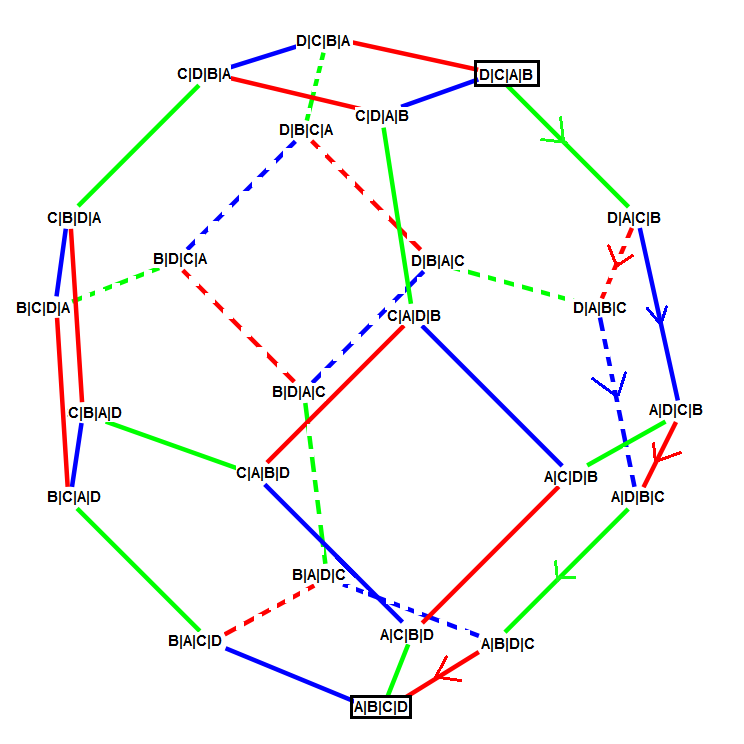
\includegraphics[width=8cm]{insert2}
\par\end{centering}

\protect\caption{\label{fig:Graphical-representation-of}Graphical representation of
weighted Kendall distance between four objects.}
\end{figure}



\subsection[The normalization constant]{The normalization constant}

The weighted Kendall distance introduced in the last section can be
formulated into a probability model. For the ranking of $t$ objects,
the model includes $t-1$ decreasing weights as well as a modal ranking
$\pi_{0}$. We refer to this new model as the weighted Kendall distance-based
model. The probability of observing a ranking $\pi$ is 
\[
\Prob(\pi|\boldsymbol{w},\pi_{0})=\frac{e^{-D_{wK}(\pi,\pi_{0})}}{C_{wK}(\boldsymbol{w})},
\]
where $C_{wK}(\boldsymbol{w})$ is the normalization constant. Although
the distance term in the model can be computed efficiently, the exact
probability would still be intractable if the normalization constant
does not have a closed form. Fortunately due to the special structure
of the model we show that $C_{wK}(\boldsymbol{w})$ has a closed form
and is given as follows. 
\begin{equation}
C_{wK}(\boldsymbol{w})=\prod_{i=1}^{t-1}\left[1+\sum_{j=1}^{i}e^{-\sum_{k=j}^{i}w_{t-k}}\right].\label{eq:4}
\end{equation}
The derivation can be found in Appendix A.


\section[Extension of distance-based models]{Extension of distance-based models}


\subsection[Finite mixture of distance-based models]{Mixture of distance-based models\label{sub:Finite-mixture-of}}

Introducing additional parameters into the distance-based ranking
models increases the flexibility of the models. However, all the models
presented in the previous sections are strongly unimodal. Fortunately
these models can be easily extended to a finite mixture of several
distance-based component models in order to cater for the heterogeneity
of the rank-order preferences among the raters. Each component model
may represent a different group of raters with their own favorite/modal
ranking ($\pi_{0,g}$) and weights ($\boldsymbol{w}_{g}$) used in
the distance function. The mixture model of $G$ components can be
defined as:
\[
\Prob(\pi_{i})=\sum_{g=1}^{G}p_{g}\Prob(\pi_{i}|\boldsymbol{w}_{g},\pi_{0,g}),
\]
where $p_{g}$ is proportion of raters in the $g$th component.

\citet{Murphy2003} first applied the EM-algorithm to efficiently
fit such mixture models. We introduce latent variables $z$ to record
the component membership of each observation. The latent (membership)
variable $z=(z_{1},z_{2},\ldots,z_{G})$ is defined such that $z_{g}$
= 1 if the observation certainly belongs to component $g$ and $z_{g}=0$
otherwise. The EM-algorithm is summarized in the following steps:

\begin{algorithm}[H]
\begin{centering}
\begin{minipage}[t]{0.95\columnwidth}%
\begin{enumerate}
\item E-Step: compute the value of $z_{g}$ for each observation $i$:
\[
\hat{z}_{g}^{(i)}=\frac{p_{g}\Prob(\pi^{(i)}|\boldsymbol{w}_{g},\pi_{0,g})}{\sum_{g'=1}^{G}p_{g'}\Prob(\pi^{(i)}|\boldsymbol{w}_{g'},\pi_{0,g'})}
\]

\item M-Step: for each component $g$, estimate $\pi_{0,g}$ and $w_{g}$
in the same way as for the case of single component except that each
observation $i$ has a 'discounted' frequency $\hat{z}_{g}^{(i)}$. 
\item Repeat the above steps until convergence.\end{enumerate}
%
\end{minipage}
\par\end{centering}

\protect\caption{EM-algorithm for fitting mixture models}
\end{algorithm}



\subsection[Top-q rankings]{Top-$q$ rankings\label{sub:Top--rankings}}

If the raters evaluate all objects but only report the rankings of
the best $q$ objects then we obtain top-$q$ ranking data. Top-$q$
ranking data is very common when the number of objects to be ranked
is large. The top-$q$ ranking can be viewed as a missing data problem,
where additional assumptions about the structure of missing data is
needed. 

A common assumption roots in the maximum entropy principle. According
to this principle, all complete rankings that are compatible with
the observed top-$q$ ranking have the same probability to occur.
We will refer to this assumption as the \textit{equal-probability
assumption}. It follows that in terms of likelihood function, observing
a top-$q$ ranking $\pi(q)$ is equivalent to adding $\frac{1}{(t-q)!}$
observation to all complete rankings compatible with $\pi(q)$. In
this way the top-$q$ rankings are transformed into complete rankings
and any model that works for complete rankings can be applied. The
shortcoming of this approach is that if the number of compatible rankings
$(t-q)!$ is large the computational cost of transforming the data
is huge.

The proposed weighted Kendall distance model can avoid such problem
if an additional assumption is imposed. This assumption is that the
raters consider all unreported objects to be \textit{equally} bad,
or in other words, those unreported objects have tied rank $q+1$.
We will refer to this assumption as the \textit{tied-rank assumption}.
Under this assumption we are able to assign $w_{j}=0$ for all $j>q$,
which means swapping objects with rank larger than $q$ does not affect
the likelihood (since they are tied). It follows from the definition
of the weighted Kendall distance that as $w_{k}=0$ for all $k>q$,
$D_{wK}(\pi_{i},\sigma)=D_{wK}(\pi_{j},\sigma)$ for any two complete
rankings $\pi_{i}$ and $\pi_{j}$ compatible with $\pi(q)$. Therefore,
we do not need to list out all complete rankings compatible with $\pi(q)$
and simply define $D_{wK}(\pi(q),\sigma)=D_{wK}(\pi,\sigma)$ with
$w_{k}=0$ for all $k>q$ and any $\pi$ compatible with $\pi(q)$.
 

The algorithm is presented in the box ``Algorithm \ref{alg:Computing-weighted-Kendall}''.
Note that the distance computation can be optimized to have time complexity
$O(q^{2})$ and the computational cost is no longer related to the
number of objects ($t$), which is an extremely desirable property
in applications where a large number of objects are compared. We will
show in Appendix B that the normalization constant $C_{q}(\boldsymbol{w})$
for top-$q$ rankings is proportional to the normalization constant
$C_{wK}(\boldsymbol{w})$ for complete rankings. In particular $C_{q}(\boldsymbol{w})=\frac{C_{wK}(\boldsymbol{w})}{(t-q)!}$.

Note that the tied-rank assumption is stronger than the equal-probability
assumption. In some applications the tied-rank assumption may not
be valid and the resulting model would not be as good. However this
assumption greatly simplifies computation when $t-q$ is big. 

If a data set contains both complete and top-$q$ rankings for $m$
distinct values of $q$, the model can still be adapted to such heterogeneity.
We can write the likelihood of the whole data set as follows:
\begin{eqnarray}
\ell(\vec{\pi}(q_{1}),\vec{\pi}(q_{2}),\ldots,\vec{\pi}(q_{m})) & = & \log\prod_{i=1}^{m}\Prob(\vec{\pi}(q_{i}))\nonumber \\
 & = & \sum_{i=1}^{m}\left[-\sum_{k=1}^{n_{q_{i}}}D_{wK}(\pi_{k}(q_{i}),\pi_{0})-n_{q_{i}}\log(C_{q_{i}})\right]\label{eq:topq_likelihood}
\end{eqnarray}
where $\vec{\pi}(q_{i})$ is the sample of all the top-$q_{i}$ rankings
in the data set and $n_{q_{i}}$ is the sample size of $\vec{\pi}(q_{i})$.

{\footnotesize{}}
\begin{algorithm}
\begin{centering}
{\footnotesize{}}%
\begin{minipage}[t]{0.95\columnwidth}%
\texttt{for r in 1 to q:}

\texttt{\ \ \ \ obj = the object with rank r in pi\_1}

\noindent \texttt{\ \ \ \ pos = UNFOUND}

\texttt{\ \ \ \ for r2 in 1 to q:}

\texttt{	\ \ \ \ if obj has rank r2 in pi\_2:}

\texttt{	\ \ \ \ \ \ \ \ pos = r2}

\texttt{\ \ \ \ if pos == UNFOUND:}

\texttt{	\ \ \ \ increment each weight}

\texttt{	\ \ \ \ increment the rank of each remaining object in
pi\_2}

\texttt{\ \ \ \ else:}

\texttt{	\ \ \ \ for j in r to (pos-1):}

\texttt{	\ \ \ \ \ \ \ \ increment weight j}

\texttt{	\ \ \ \ \ \ \ \ increment rank j in pi\_2}

\texttt{return weight}%
\end{minipage}
\par\end{centering}{\footnotesize \par}

{\footnotesize{}\protect\caption{\label{alg:Computing-weighted-Kendall}Computing weighted Kendall
distance between top-$q$ rankings}
}
\end{algorithm}
{\footnotesize \par}


\section[Package design and implementation]{Package architecture and implementation}

The \pkg{rankdist} package is available from the Comprehensive \proglang{R}
Archive Network (CRAN) at \url{http://CRAN.R-project.org/package=rankdist}.
The latest development version can be found at \url{https://github.com/ZhaozhiQIAN/rankdist}.
The software is written in \proglang{R} and \proglang{C++}.


\subsection[Existing software]{Existing software for modelling ranking data}

At present, there are several alternative packages for modeling ranking
data in \proglang{R} including \pkg{PerMallows} \citep{PerMallows},
\pkg{rankcluster} \citep{Rankcluster}, \pkg{pmr} \citep{pmr} and
\pkg{mlogit} \citep{mlogit}. 

Package \pkg{PerMallows} implements six common distance-based models.
The software is primarily written in \proglang{C++} but it includes
an interface to \proglang{R}. The key features that distinguish \pkg{rankdist}
from \pkg{PerMallows} are (1) the support for mixture models; (2)
the more compact representation of ranking data set; and (3) extendability.
Package \pkg{PerMallows} employs keyword matching in determining
the model to use. In order to add a new model, the developer has to
both implement the model and change the callers' code as well. \pkg{rankdist}
is designed differently so that no modifications are needed for the
caller. Package \pkg{PerMallows} has two functionality that are currently
unavailable in \pkg{rankdist}. It contains abundant utility functions
to perform calculations related to permutations and it includes different
ways to draw samples from the fitted model. 

Package \pkg{rankcluster} is able to fit mixture models for ranking
data. It only supports the ISR model \citep{ISR}. Package \pkg{pmr}
includes four distance-based ranking models and their weighted version.
It currently does not support mixture models. Package \pkg{mlogit}
implements the mixed logit model and multinomial probit model, which
belong to the order-statistics models \citep{AlvoYu2014}. These packages use different
data structures to represent and store ranking data and fitted models. 


\subsection[Package architecture]{Package architecture}

The package \pkg{rankdist} is designed with efficiency and extendability
in mind. Where possible, \proglang{C++} code is used to perform computationally
intensive steps. The \proglang{R} code is optimized to reduced memory
footprints. The package is carefully modularized. Making modifications
on one part of the software is unlikely to affect the other parts.
Unit tests are also implemented in order to avoid code degradation. 

Three \proglang{S4} classes serve as the backbone of the package.
The \code{RankData} class keeps all the information about the ranking
data set. The \code{RankInit} class specifies initial parameter settings
and indicates whether we want to fit a mixture model. The \code{RankControl}
class is a void class and it has to be derived into a \code{RankControl[model]}
class. This class specifies which model we want to fit and the control
parameters used in the optimization procedure.

The flowchart in Figure \ref{fig:flowchart} illustrates the model
fitting procedure. Three input objects are provided to the model generator
function \code{RankDistanceModel}. This function will apply the EM
solver if the \code{RankInit} object contains initial values for
more than one component. As discussed in Section \ref{sub:Finite-mixture-of},
each component model in the mixture is fitted to a ranking data set
with ``discounted'' observations. In fact the EM solver will prepare
those data sets and make multiple calls to \code{SearchPi0}, which
fits a single component model. The function \code{SearchPi0} then
searches the optimum modal rankings. The details of this algorithm
is described in Section \ref{sub:Estimation-pi0}. Checked candidates
are cached in a hash table to prevent double checking. For each candidate
modal ranking, the function \code{SingleClusterModel} is called to
estimate parameter weightings. It is implemented as a generic function
and the internal method dispatch mechanism will apply suitable solver
according to the signature of the \code{RankControl[model]} object. 

\begin{figure}[h]
\begin{centering}
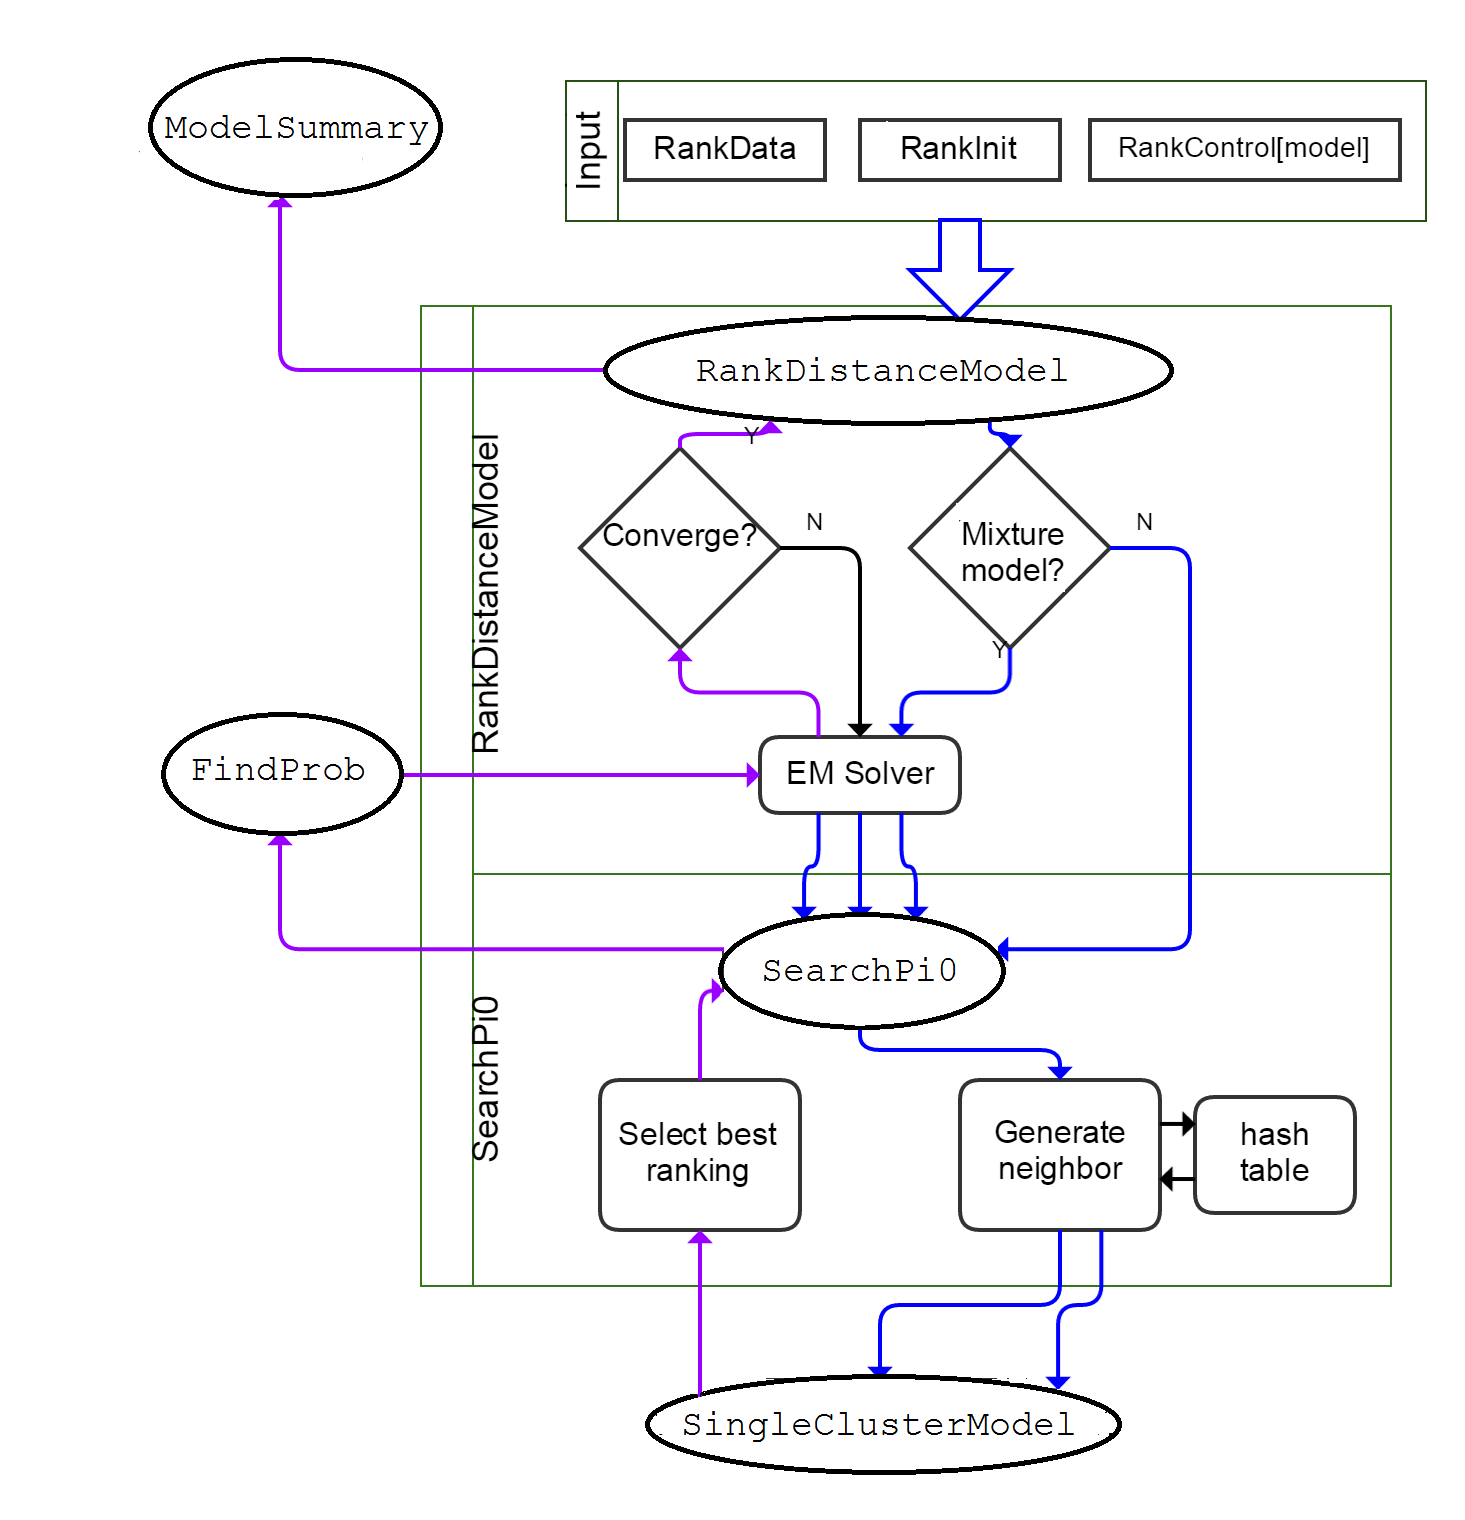
\includegraphics[scale=0.5]{flowchart}
\par\end{centering}

\protect\caption{\label{fig:flowchart}Flow chart of the model fitting procedure.}
\end{figure}
The purple arrows illustrate how the functions return values. \code{SingleClusterModel}
returns fitted parameters and log-likelihood. \code{SearchPi0} selects
the modal ranking according to the log-likelihood. Another generic
function \code{FindProb} is called to give the fitted probabilities
of observed rankings. Similar to \code{SingleClusterModel}, this
function is also model dependent. The EM solver updates each component
data set according to these fitted probabilities. The \code{RankDistanceModel}
function returns the final model if EM algorithm converges or a single
component model is required. The function \code{ModelSummary} can
display the parameters in the fitted model in a clear way.

The object-oriented approach brings two immediate benefits. First
of all, the ranking data stored in the data structure are better protected
against user mistakes such as confusing rankings with orderings. The
data integrity benefits as a result. Secondly, with a higher level
of abstraction implementing a new ranking model reduces to extending
the \code{RankControl} class and implementing the two methods (\code{SingleClusterModel}
and \code{FindProb}), and the other parts of the software do not
need to be affected. Such infrastructure can be used in other packages
which deal with ranking data. We hope the package would make experiments
with new ranking models easier.


\subsection[Estimation of weights]{Estimation of weights \label{sub:Estimation-of-weights}}

For models that utilize unweighted distance metric as defined in (\ref{eq:dist_model_def})
there is only one free parameter, namely the dispersion parameter
$\lambda$. The log-likelihood function of such model will become:
\[
\ell(\pi_{1},\pi_{2},...,\pi_{n})=-\lambda\sum_{i=1}^{n}D(\pi_{i},\pi_{0})-n\log(C).
\]
Given $\pi_{0},$ one dimensional optimization techniques can then
be used to determine the maximum likelihood estimate of $\lambda$.
In the package we use \code{optimize} function in \proglang{R} to
implement this \citep{R}.

For the $\phi$-component model defined in (\ref{eq:phi_component})
or equivalently (\ref{eq:phi_component_simp}), the log-likelihood
function will be:
\[
\ell(\pi_{1},\pi_{2},...,\pi_{n})=-\sum_{j=1}^{t-1}\left[\sum_{i=1}^{n}\lambda_{j}\cdotp V_{j}(\pi_{i},\pi_{0})-n\log(C_{j}(\lambda_{j}))\right].
\]
Therefore the maximization of log-likelihood function over $t-1$
parameters is reduced to maximizing $t-1$ independent one-dimensional
functions. The package also uses \code{optimize} function in \proglang{R}
to implement this.

For the weighted tau model, the optimization cannot be simplified
into a series of one-dimensional optimization, and the gradient function
of the log-likelihood function is also intractable. Hence, the Nelder-Mead
method available in the \proglang{R} package \pkg{Optimx} is used
\citep{nash2011unifying}. 

For the weighted Kendall model the log-likelihood function is given
by:

\[
\ell(\pi_{1},\pi_{2},...,\pi_{n})=-\sum_{i=1}^{n}\sum_{j=1}^{t-1}w_{j}Q_{j}(\pi_{i},\pi_{0})-n\log(C_{wK}(\boldsymbol{w})),
\]
where $Q_{j}(\pi_{i},\pi_{0})$ is defined as in (\ref{eq:3}). Maximizing
the log-likelihood function under the decreasing constraint on $w$
can be difficult. Instead, we reparametrize $w_{j}$ as $w_{j}=\sum_{i=j}^{t-1}\phi_{i}$,
where $\phi_{i}\geq0$ for all $i$, and thus transform a complicated
constraint into a box constraint. The log-likelihood function can
be rewritten as:
\[
\ell(\pi_{1},\pi_{2},...,\pi_{n})=-\sum_{i=1}^{n}\sum_{j=1}^{t-1}\phi_{j}\left[\sum_{k=j}^{t-1}Q_{k}(\pi_{i},\pi_{0})\right]-n\log(C_{wK}(\boldsymbol{w}(\boldsymbol{\phi}))).
\]


Given $\pi_{0},$ the partial derivatives of the log-likelihood function
with respect to $\phi$ have analytical forms and can be determined
efficiently. Quasi-Newton methods which support box constraints can
be used to determine the maximal value of $\phi$ given $\pi_{0}$.
The L-BFGS-B method in the \proglang{R} package \pkg{Optimx} is
used for such optimization. 

The optimization algorithm require initial values of $\phi$. In order
to make an educated guess of initial values of $\phi$, we can utilize
the following equation
\[
\log(\frac{P(\pi_{u})}{P(\pi_{v})})=-\sum_{i=1}^{n}\sum_{j=1}^{t-1}\left[\sum_{k=j}^{t-1}Q_{k}(\pi_{u},\pi_{0})\right]\cdot\phi_{j}+\sum_{i=1}^{n}\sum_{j=1}^{t-1}\left[\sum_{k=j}^{t-1}Q_{k}(\pi_{v},\pi_{0})\right]\cdot\phi_{j}
\]


Sample $k$ pairs of <$\pi_{u},\pi_{v}$> from observed data and replace
the corresponding probabilities with observed proportions. The result
will be a overdetermined system of $k$ linear equations involving
$\phi$. Linear least square method can be used to solve for $\phi$
and the resulting values are set as the initial values.


\subsection[Estimation of the central ranking]{Estimation of the central ranking\label{sub:Estimation-pi0}}

Searching for the optimal value of $\pi_{0}$ is a well-known difficult
problem. We set the initial value of $\pi_{0}$, denoted as $\pi_{00}$.
This initial value could be randomly selected or we can use a frequently
observed ranking. Then all its neighboring rankings are considered
and their log-likelihoods are calculated. If $\pi_{00}$ achieves
the largest likelihood then we stop. Otherwise, we select the one
with the largest likelihood as $\pi_{01}$ and consider all of its
neighbors again. This process repeats until $\pi_{0k}$ has larger
likelihood than all its neighbors. 

The neighboring rankings are defined as all rankings adjacent to the
current ranking with respect to Cayley or Kendall distance. The user
can choose either measure according to the availability of computation
resources. 


\section[Using the rankdist package]{Using the \pkg{rankdist} package}


\subsection[Preprocessing]{Preprocessing}

The ranking data can have two equivalent representations: ranking
and ordering. The ranking representation records the ranks of objects
in the form $(\pi(1),\,\pi(2),\ldots)$ where $\pi(i)$ is the rank
of object $i$ while the ordering representation records the objects
in the rank order $(\pi^{-1}(1),\,\pi^{-1}(2),\ldots)$ where $\pi^{-1}(i)$
is the object ranked the $i$th. Since both representations are common,
it is very important for us to make a clear distinction and avoid
any confusion. The \pkg{rankdist} package stores ranking data in
a \proglang{S4} class \code{RankData}. The user only need to initialize
the object once using either representation and the software would
handle the internal data storage problem implicitly. The details of
the \code{initialize} method of \code{RankData} class can be found
in the full documentation that is available as part of the software.

In the following example the \code{GenerateExample} function generate
independent samples from the same distribution, but the data representation
depends on the argument \code{ranking=TRUE}. The sample contains
the rankings of five objects and the underlying model is a Mallows'
$\phi$ model with parameter $\lambda=0.2$ and the modal ranking
$\pi_{0}=(1,2,3,4,5)$. Note that the \code{ranking} or \code{ordering}
matrix cannot have duplicated rows and the number of observations
for each ranking is specified in a vector \code{count}.

\begin{CodeChunk}
\begin{CodeInput}
R> library("rankdist")
R> gen1<- GenerateExample(ranking=TRUE) 
R> tail(gen1$ranking)
\end{CodeInput}
\begin{CodeOutput}
       [,1] [,2] [,3] [,4] [,5]
[115,]    5    4    1    2    3
[116,]    5    4    1    3    2
[117,]    5    4    2    1    3
[118,]    5    4    2    3    1
[119,]    5    4    3    1    2
[120,]    5    4    3    2    1
\end{CodeOutput}
\begin{CodeInput}
R> dat1 <- new("RankData", ranking=gen1$ranking, count=gen1$count)
R> gen2 <- GenerateExample(ranking=FALSE) 
R> tail(gen2$ordering)
\end{CodeInput}
\begin{CodeOutput}
       [,1] [,2] [,3] [,4] [,5]
[115,]    3    4    5    2    1 
[116,]    3    5    4    2    1 
[117,]    4    3    5    2    1 
[118,]    5    3    4    2    1 
[119,]    4    5    3    2    1 
[120,]    5    4    3    2    1
\end{CodeOutput}
\begin{CodeInput}
R> dat2 <- new("RankData", ordering=gen2$ordering, count=gen2$count)
\end{CodeInput}
\end{CodeChunk}

The user can also store a data set that contains top-$q$ rankings.
Two additional arguments needs to be provided. The \code{GenerateExampleTopQ}
function generates top-three rankings of five objects.

\begin{CodeChunk}
\begin{CodeInput}
R> genq <- GenerateExampleTopQ() 
R> head(genq$ranking)
\end{CodeInput}
\begin{CodeOutput}
     [,1] [,2] [,3] [,4] [,5]
[1,]    1    2    3    4    4
[2,]    1    2    4    3    4
[3,]    1    2    4    4    3
[4,]    1    3    2    4    4
[5,]    1    3    4    2    4
[6,]    1    3    4    4    2
\end{CodeOutput}
\begin{CodeInput}
R> datq <- new("RankData", ranking=genq$ranking, count=genq$count, 
+           nobj=5, topq=3) 
\end{CodeInput}
\end{CodeChunk}


\subsection[Model generation]{Model generation}

We specify which model we are going to use by creating a control object
that inherits from \code{RankControl}. Suppose we are going to use
Mallows' $\phi$ model and weighted Kendall model. Additional parameters
can be provided to specify the behavior of the parameter estimation,
the search for modal ranking and the EM algorithm. 

\begin{CodeChunk}
\begin{Code}
R> ctrl1 <- new("RankControlKendall", SearchPi0_show_message=FALSE)
R> ctrlq <- new("RankControlWeightedKendall", SearchPi0_show_message=FALSE) 
\end{Code}
\end{CodeChunk}

Since the parameter estimation requires the initial values of parameters,
we need to specify these in a \code{RankInit} object. The function
\code{MomentsEst} gives a heuristic estimate of the initial values
as explained in Section \ref{sub:Estimation-of-weights}. We can also
use the software to fit a mixture model.

\begin{CodeChunk}
\begin{Code}
R> str1 <- MomentsEst(dat1, 500)
R> init1 <- new("RankInit", param.init=list(str1),
+            modal_ranking.init=list(1:5), clu=1L) 
R> init1c <- new("RankInit", param.init=list(str1,str1),
+            modal_ranking.init=list(1:5,5:1), clu=2L)
R> initq <- new("RankInit", param.init=list(rep(0.5,3)),
+            modal_ranking.init=list(1:5), clu=1L) 
\end{Code}
\end{CodeChunk}

After that, the model generation is done by the generic function \code{RankDistanceModel} 

\begin{CodeChunk}
\begin{Code}
R> model1 <- RankDistanceModel(dat1, init1, ctrl1) 
R> model1c <- RankDistanceModel(dat1, init1c, ctrl1) 
R> modelq <- RankDistanceModel(datq, initq, ctrlq)
\end{Code}
\end{CodeChunk}

We can have a summary of the fitted model by calling the \code{ModelSummary}
function. Two common approaches to assess the goodness of fit of a
particular model is the BIC value and the sum of squares of Pearson
residuals (SSR). 
\[
BIC=-2\cdotp\ell(\pi_{1},\pi_{2},...,\pi_{n})+dof\cdotp\log(n)
\]
\[
SSR=\sum_{i=1}^{t!}\frac{(O_{i}-E_{i})^{2}}{E_{i}},
\]
where $dof$ is the number of free parameters in the model and $O_{i}$
and $E_{i}$ are the observed and expected frequencies of the $i$th
ranking, respectively. A lower value in BIC and SSR indicates a better
fit. 

\begin{CodeChunk}
\begin{CodeInput}
R> ModelSummary(model1)
\end{CodeInput}
\begin{CodeOutput}
Summary of model1
================ 
Goodness of Fit 
SSR:	 109.426  
BIC:	 -18832.76  
dof:	 1  
Parameter Estimation 
Cluster  A  B  C  D  E  p  Parameters 
1        1  2  3  4  5  1  0.2	
\end{CodeOutput}
\begin{CodeInput}
R> ModelSummary(model1c)
\end{CodeInput}
\begin{CodeOutput}
Summary of model1c  
================= 
Goodness of Fit
SSR:	 107.5339  
BIC:	 -18847.38  
dof:	 3  
Parameter Estimation 
Cluster  A  B  C  D  E  p   Parameters 
1        1  2  3  4  5 0.72   0.26	 
2        2  1  5  4  3 0.28   0.08	
\end{CodeOutput}
\begin{CodeInput}
R> ModelSummary(modelq)
\end{CodeInput}
\begin{CodeOutput}
Summary of modelq  
================ 
Goodness of Fit 
SSR:	 48.86542  
BIC:	 -90590.52  
dof:	 3  
Parameter Estimation 
Cluster  A  B  C  D  E  p  Parameters 
1        1  2  3  4  4  1  0.7  0.52  0.28  0
\end{CodeOutput}
\end{CodeChunk}


\section[Experimental study]{Experimental study}


\subsection[Modeling ranking probability]{Modeling ranking probability}


\subsubsection[Data set and methodology]{Data set and methodology}

The APA Election data set consists of $15,449$ votes in the 1980
American Psychological Association (APA) presidential election \citep{Diaconis1988}.
There are $5,738$ complete rankings and there are five candidates
in the election. This data set is well studied in the literature and
it has been included in the \pkg{rankdist} package. We use this data
set to illustrate various ranking models available in the package.


In the experiment we consider the following distance-based ranking
models available in the \pkg{rankdist} package: 
\begin{itemize}
\item Mixture of Mallows' $\phi$ model (Section \ref{sub:Mallows'--model})
\item Mixture of weighted tau model (Section \ref{sub:Weighted-Kendall-distance-model})
\item Mixture of weighted Kendall model proposed in this paper (Section
\ref{sec:Geometrically-weighted-Kendall})
\end{itemize}
For single-parameter models we fit a mixture of up to eight components
and for more complicated models we fit up to three components. The
BIC criterion is used to select the best number of components in the
mixture model by choosing the one with the smallest BIC. Multiple
initial value configurations have been tried in order to avoid convergence
to local maximal value. 


\subsubsection{Modeling for the complete rankings}

The following code snippet illustrates the way to fit mixtures of
weighted Kendall distance-based model to APA election data set using
the \pkg{rankdist} package. Fitting other types of distance-based
models is similar.

\begin{CodeChunk}
\begin{CodeInput}
R> library("rankdist") 
R> apa_wk_ctrl<-new("RankControlWeightedKendall",
+	SearchPi0_fast_traversal=TRUE, SearchPi0_show_message=FALSE) 
R> wKendall_model <- list() 
R> for (i in 1L:3L){ 
R>   init <- new("RankInit", param.init=replicate(i, 0.1, FALSE),
+		modal_ranking.init=replicate(i, sample(5,5), FALSE),
+		clu=i, p.init=rep(1,i)/i) 
R>   wKendall_model[[i]] <- RankDistanceModel(apa_obj, init, apa_wk_ctrl) 
R> }
\end{CodeInput}
\end{CodeChunk}

We present the model fitting results in Tables \ref{tab:Summary-of-mod}
and \ref{tab:Parameters-of-mod}. Table \ref{tab:Summary-of-mod}
displays the best fitted models selected using the BIC criterion while
Table \ref{tab:Parameters-of-mod} shows the parameter estimates of
the three fitted models. It can be seen that the weighted Kendall
model achieves the best fit in terms of BIC and SSR.

\begin{table}[h]
\begin{centering}
\begin{tabular}{|c|c|c|c|c|}
\hline 
Model & Components & Free Parameters & BIC & SSR\tabularnewline
\hline 
\hline 
Weighted Kendall & 3 & 9 & 53685.4 & 398.00\tabularnewline
\hline 
Mallows' $\phi$  & 5 & 9 & 53729.3  & 444.24\tabularnewline
\hline 
Weighted tau & 3 & 17 & 53785.2 & 421.44\tabularnewline
\hline 
\end{tabular}
\par\end{centering}

\protect\caption{\label{tab:Summary-of-mod}Summary of the fitted models for complete
rankingss}
\end{table}


There are several well-known facts about the APA election data set.
First, candidates A and C are research psychologists, candidates D
and E are clinical psychologists and candidate B is a community psychologist.
Candidates naturally form three competing subgroups, and voters show
different preferences towards different subgroups. We can see from
Table \ref{tab:Parameters-of-mod} that the model based on weighed
Kendall distance forms three clusters. Based on the estimates of the
modal rankings of the three clusters, candidates A and C ranked at
the top two in the first cluster while candidates D and E are preferred
in the second cluster, and the third cluster assigns the highest rank
to candidate E. The competing effects between different candidates
are obvious. The weighted tau model does not capture this phenomenon
although a three-component mixture model is found. The Mallows' $\phi$
model captures the competing relationship with the first two clusters,
but it also includes a few smaller but confounding components. The
inflexibility of single-parameter models often requires a larger number
of mixing components, which makes interpretation more difficult.

The new model also allows more fine-grained interpretation. The weights
for swapping first three positions are higher in the first cluster
than the second cluster. This suggests that for those who prefer candidates
A and C, they have a stronger tendency to do so. On the contrary,
the weights for the third cluster is lower, suggesting that voters
in this cluster have more diverse preferences. 

\begin{table}
\begin{centering}
\begin{tabular}{|c|c|c|c|c|c|c|c|c|c|c|c|c|}
\hline 
\multirow{2}{*}{Model} & \multirow{1}{*}{Cluster} & \multicolumn{5}{c|}{Modal ranking $\pi_{0g}$} & \multirow{2}{*}{$w_{1g}$} & \multirow{2}{*}{$w_{2g}$} & \multirow{2}{*}{$w_{3g}$} & \multirow{2}{*}{$w_{4g}$} & \multirow{2}{*}{$w_{5g}$} & Proportion\tabularnewline
\cline{3-7} 
 & $g$ & A & B & C & D & E &  &  &  &  &  & $p_{g}$\tabularnewline
\hline 
\hline 
\multirow{3}{*}{Weighted Kendall} & 1 & 2 & 3 & 1 & 5 & 4 & 1.02 & 1.02 & 0.51 & 0.33 & - & 37\%\tabularnewline
\cline{2-13} 
 & 2 & 3 & 4 & 5 & 1 & 2 & 0.47 & 0.47 & 0.35 & 0.35 & - & 33\%\tabularnewline
\cline{2-13} 
 & 3 & 4 & 2 & 5 & 3 & 1 & 0.23 & 0.21 & 0.21 & 0.21 & - & 30\%\tabularnewline
\hline 
\hline 
\multirow{5}{*}{Mallows' $\phi$ } & 1 & 3 & 2 & 5 & 1 & 4 & 0.38 & - & - & - & - & 27\%\tabularnewline
\cline{2-13} 
 & 2 & 2 & 3 & 1 & 5 & 4 & 0.83 & - & - & - & - & 25\%\tabularnewline
\cline{2-13} 
 & 3 & 3 & 4 & 5 & 1 & 2 & 0.61 & - & - & - & - & 21\%\tabularnewline
\cline{2-13} 
 & 4 & 3 & 4 & 2 & 5 & 1 & 0.24 & - & - & - & - & 20\%\tabularnewline
\cline{2-13} 
 & 5 & 2 & 5 & 1 & 3 & 4 & 0.72 & - & - & - & - & 8\%\tabularnewline
\hline 
\hline 
\multirow{3}{*}{Weighted tau} & 1 & 2 & 3 & 5 & 1 & 4 & 1.72 & 0 & -0.99 & -0.28 & 0.39 & 40\%\tabularnewline
\cline{2-13} 
 & 2 & 5 & 2 & 4 & 1 & 3 & 3.65 & 0.91 & -0.08 & 0.1 & -0.04 & 31\%\tabularnewline
\cline{2-13} 
 & 3 & 1 & 2 & 4 & 3 & 5 & 1.78 & 0.58 & -0.36 & -1.14 & -0.58 & 29\%\tabularnewline
\hline 
\end{tabular}
\par\end{centering}

\protect\caption{\label{tab:Parameters-of-mod}Parameter estimates of the fitted models
for complete ranking.}


\end{table}


We apply a mulitdimensional scaling (MDS) to the $120\times120$ distance
matrix with each cell being the Kendall distance between two observed
rankings. Figure \ref{fig:Visualization-of-APA} shows a plot of the
two-dimensional solution to MDS. Each point on the plot represents
a ranking. The distance between points on the plot is approximately
proportional to the Kendall distance between two corresponding rankings.
The size of the point represents the observed frequency of the ranking,
whereas the color represents the expected frequency from the fitted
weighted Kendall model. 

\begin{figure}[h]
\begin{centering}
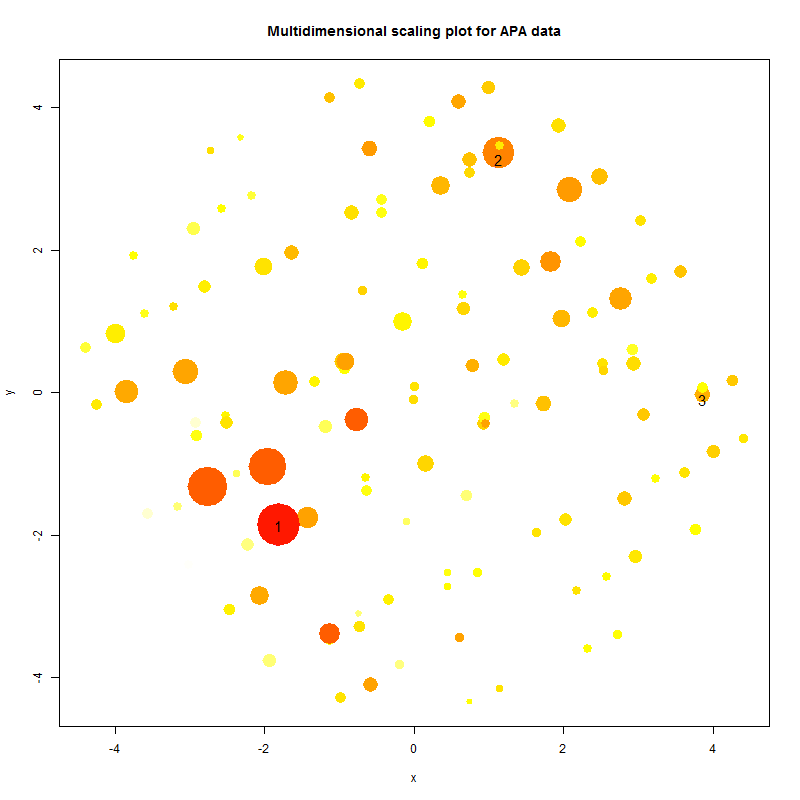
\includegraphics[scale=0.6]{MDS_APA}
\par\end{centering}

\protect\caption{\label{fig:Visualization-of-APA}Visualization of APA data with fitted
model.}
\end{figure}


It can be observed that larger points often have darker color, which
indicates the expected frequencies agree with observed ones. The modal
rankings of the three clusters are labeled as 1, 2 and 3 on the plot.
The first two clusters in the model are clearly reflected on the plot
as two distinct regions of larger points whereas the structure of
the third cluster looks a bit less clear. As mentioned before, voters
in the third cluster have more diversified opinions. It is thus reasonable
that there are few dominating rankings in this cluster and the cluster
looks more noisy. 


\subsubsection{Modeling for All Rankings}

In the APA election data set, there are 5,738 complete rankings and
9,711 incomplete rankings. Analysis based on the data with the incomplete
rankings removed may have a significant effect on the conclusion drawn
from the data. Here, we fit weighted Kendall model to all rankings.
Both the equal probability and tied rank assumptions described in
Section \ref{sub:Top--rankings} are considered in the estimation
of the model parameters.

Since the number of objects in APA election data set is only $5$,
there would not be any computational burden even if the equal probability
assumption is used. As the equal probability assumption is weaker
than the tied rank assumption, it is more likely to generate a better
fit model to the data. Tables \ref{tab:sum-all} and \ref{tab:Parameters-of-all}
show the best fitted mixture models under the two assumptions and
the parameter estimates of these models. 

\begin{table}[H]
\centering{}%
\begin{tabular}{|c|c|c|c|c|}
\hline 
Assumption & Components & Free Parameters & BIC & SSR\tabularnewline
\hline 
\hline 
Equal probability & 3 & 10 & 141276.5 & 1420.64 \tabularnewline
\hline 
Tied rank & 3 & 9 & 141479.5 & 1615.97\tabularnewline
\hline 
\end{tabular}\protect\caption{\label{tab:sum-all}Summary for the fitted models for all rankings.}
\end{table}


\begin{table}[H]
\centering{}%
\begin{tabular}{|c|c|c|c|c|c|c|c|c|c|c|c|}
\hline 
\multirow{2}{*}{Assumption} & Cluster & \multicolumn{5}{c|}{Modal ranking $\pi_{0g}$} & \multirow{2}{*}{$w_{1g}$} & \multirow{2}{*}{$w_{2g}$} & \multirow{2}{*}{$w_{3g}$} & \multirow{2}{*}{$w_{4g}$} & Proportion\tabularnewline
\cline{3-7} 
 & $g$ & A & B & C & D & E &  &  &  &  & $p_{g}$\tabularnewline
\hline 
\hline 
\multirow{3}{*}{Equal probability} & 1 & 3 & 4 & 5 & 1 & 2 & 0.40 & 0.40 & 0.24 & 0.17 & 44\%\tabularnewline
\cline{2-12} 
 & 2 & 2 & 3 & 1 & 5 & 4 & 1.08 & 1.08 & 0.37 & 0.22 & 29\%\tabularnewline
\cline{2-12} 
 & 3 & 3 & 1 & 5 & 4 & 2 & 0.19 & 0.19 & 0.15 & 0.15 & 27\%\tabularnewline
\hline 
\hline 
\multirow{3}{*}{Tied rank} & 1 & 3 & 4 & 5 & 2 & 1 & 0.52 & 0.52 & 0.41 & 0.03 & 43\%\tabularnewline
\cline{2-12} 
 & 2 & 2 & 1 & 5 & 3 & 4 & 0.27 & 0.27 & 0.27 & 0.03 & 32\%\tabularnewline
\cline{2-12} 
 & 3 & 2 & 3 & 1 & 5 & 4 & 1.75 & 1.75 & 0.26 & 0.26 & 25\%\tabularnewline
\hline 
\end{tabular}\protect\caption{\label{tab:Parameters-of-all}Parameter estimates of the fitted models
for all rankings.}
\end{table}


It can be seen from Table \ref{tab:sum-all} that both models suggest
a 3-component solution but the fitted model based on the equal probability
assumption has a better fit in terms of BIC and SSR even though it
has one parameter more than the fitted model based on the tied rank
assumption.

Note that more than 60\% of data are incomplete rankings. After fitting
the weighted Kendall models (with equal probability assumption) to
all rankings, the results are slightly different from those for complete
rankings. It is found from Table \ref{tab:Parameters-of-all} that
the largest cluster (44\%) becomes the one with candidates D and E
ranked at the top two and the one with candidates A and C ranked at
the top two is the next largest cluster (29\%). This indicates that
the voters who gave incomplete rankings tend to prefer candidates
D and E more. Finally, the third cluster represents about 27\% of
voters who have diverse views on their favorable candidates.


\subsection[Rank aggregation]{Rank aggregation}

The problem of rank aggregation is to combine the rankings of objects
given by a panel of judges. Typical applications can be found in many
fields including social sciences, bioinformatics, meta search studies
and sport competitions. \citet{Klementiev2008} suggested using Mallows'
$\phi$ model to aggregate complete/incomplete rankings. The problem
can then be often formulated as the following optimization task

\[
\pi^{*}=\argmin\left\{ \sum_{i}D_{K}(\pi_{i},\pi^{*})\right\} .
\]


However, finding the global optimal aggregated ranking can be very
computationally intensive. In fact, it has been shown that the above
problem is NP-hard \citep{KemedyNP}. Instead of using Kendall distance,
we can fit the weighted Kendall model to the data and use the estimated
modal ranking to be the aggregated ranking. 

In this section, we test whether the weighted Kendall distance model
fitted by the greedy search scales up well and provides reasonable
results. We compare the result with the ground truth and the aggregated
ranking given by Borda Count method \citep{Marden1995a}, which is
based on the arithmetic mean of the observed rankings.

We applied the model to 20 different data sets collected by \citet{lee2014cognitive}
where undergraduates recruited from the human subjects pool at the
University of California Irvine were asked to perform 20 ranking tasks.
The ranking tasks involve either general knowledge of existing ground
truths or predictions of future outcomes. As the true rankings of
the objects are finally known in all 20 tasks, we can assess the goodness
of the aggregated ranking given by the estimated modal ranking of
the fitted weighted Kendall model. 

The data sets and the model performance are summarized in Table \ref{tab:Rank-Aggregation-Results}.
All data sets involve around 10 objects and fewer than 150 observations.
The column ``BetterObs'' of Table \ref{tab:Rank-Aggregation-Results}
records the percentage of observed rankings which are closer to the
true ranking than the aggregated ranking in terms of Kendall distance.
The column ``DistToTruth'' records the Kendall distance between
the true ranking and the aggregated ranking. The last column records
the Kendall distance between the true ranking and the ranking obtained
from Borda Count method. 

\begin{table}
\centering{}%
\begin{tabular}{|c|c|c|c|c|c|}
\hline 
Data Set Name & Nobj & Nobs & BetterObs & DistToTruth & BordaToTruth\tabularnewline
\hline 
Nine of Ten Amendments  & 9 & 63 & 0\% & 1 & 1\tabularnewline
\hline 
Book Releases  & 10 & 78 & 12\% & 6 & 7\tabularnewline
\hline 
Classic Oscar Releases  & 10 & 78 & 10\% & 4 & 3\tabularnewline
\hline 
Country Landmasses  & 10 & 142 & 0\% & 1 & 1\tabularnewline
\hline 
Country Populations  & 10 & 78 & 18\% & 11 & 11\tabularnewline
\hline 
European City Populations  & 10 & 78 & 24\% & 12 & 11\tabularnewline
\hline 
Hardness of Materials  & 10 & 78 & 28\% & 13 & 11\tabularnewline
\hline 
Movie Releases  & 10 & 78 & 1\% & 1 & 2\tabularnewline
\hline 
Recent Oscar Releases  & 10 & 78 & 0\% & 1 & 4\tabularnewline
\hline 
River Lengths  & 10 & 78 & 15\% & 12 & 11\tabularnewline
\hline 
Super bowl  & 10 & 78 & 3\% & 8 & 10\tabularnewline
\hline 
Ten Amendments  & 10 & 78 & 5\% & 4 & 6\tabularnewline
\hline 
Ten Commandments  & 10 & 78 & 12\% & 9 & 12\tabularnewline
\hline 
US City Populations  & 10 & 142 & 1\% & 6 & 2\tabularnewline
\hline 
US Holidays  & 10 & 146 & 0\% & 0 & 2\tabularnewline
\hline 
US Presidents  & 10 & 142 & 0\% & 0 & 0\tabularnewline
\hline 
US States West to East  & 10 & 78 & 5\% & 2 & 3\tabularnewline
\hline 
World City Populations  & 10 & 144 & 1\% & 7 & 9\tabularnewline
\hline 
NBA East 2010 Season  & 15 & 148 & 20\% & 35 & 36\tabularnewline
\hline 
NBA West 2010 Season  & 15 & 135 & 11\% & 20 & 24\tabularnewline
\hline 
\end{tabular}\protect\caption{\label{tab:Rank-Aggregation-Results}Rank aggregation results of 20
different data sets.}
\end{table}


The rank aggregation results reveal that in most cases, only a small
fraction of observed rankings are better than the aggregated ranking.
Furthermore, in 15 out of 20 cases the aggregated ranking obtained
from the new model is closer or has the same distance to the truth
than the one obtained by Borda Count method. This indicates that the
weighted Kendall distance model generally performs better than Borda
Count methods in aggregating rankings.


\section[Conclusions]{Conclusions}

In this paper, we presented the \proglang{R} package \pkg{rankdist}
for fitting different distance-based ranking models. We also introduced
a new probability model based on weighted Kendall distance whose parametrization
allows an elegant graphical interpretation. We have shown that the
model has a nice analytical form and can be easily extended into some
more complicated forms. 

In the experimental study we have shown that the package offers a
simple and coherent way to fit a wide variety of ranking models. Model
selection and comparison are made easy as a consequence. Moreover
the package \pkg{rankdist} can be easily modified to incorporate
new ranking models. Thus it provides a platform for simulation experiments
and development of new ranking models.

We found that the computation time for model-fitting procedure is
dominated by the neighbour-checking step in the search of modal ranking.
In this step the program checks all neighbours of the current best
modal ranking. A possible way to improve the \pkg{rankdist} package
is therefore to parallelize this step and fully utilize the power
of multi-core processors. 


\section*{Acknowledgments}

The research of Philip L. H. Yu was supported by a grant from the
Research Grants Council of the Hong Kong Special Administrative Region,
China (Project No.17303515).

\bibliography{paper_ref}

\section*{Appendix}

\appendix

\section*{A. Derivation of the Normalization Constant}

Denote $S_{t}$ be the set of all possible permutations of $t$ objects
labelled by integers $\{1,\cdots,t\}$, and $\pi_{0}$ be the modal
ranking of interest. For any ranking $\pi$ in $S_{t}$, we can use
(\ref{eq:1}) to construct a vector $\vec{V}=$ $<V_{1},V_{2},\cdots,V_{t-1}>$,
where 
\[
V_{i}=\sum_{j=i+1}^{t}I\{[\pi(\pi_{0}^{-1}(i))-\pi(\pi_{0}^{-1}(j))]>0\}.
\]


Note that $V_{i}$ can take value $0,1,\cdots,t-i$. Let $\Omega=\{<V_{1},V_{2},\cdots,V_{t-1}>|V_{i}\leq t-i,V_{i}\in\mathbb{N}_{0}\}$
be the set of all possible values of the $V_{i}$'s, where $\mathbb{N}_{0}=\{0,1,2,\cdots\}$.
\citet{Fligner1988} showed that the definition of $\vec{V}$ itself
provides a bijective mapping $f:S_{t}\rightarrow\Omega$. It follows
that if the sets $\Gamma_{1},\Gamma_{2},\cdots,\Gamma_{m}$ partition
the set $\Omega$, then the sets $f^{-1}(\Gamma_{1}),f^{-1}(\Gamma_{2}),\cdots,f^{-1}(\Gamma_{m})$
partition the set $S{}_{t}$, and vice versa. 

In the first step, we partition $\Omega$ into the following two sets:
\begin{eqnarray*}
\Gamma_{1,1} & = & \{<V_{1},V_{2},\cdots,V_{t-2},1>|V_{i}\leq t-i,V_{i}\in\mathbb{N}_{0}\},\\
\Gamma_{1,0} & = & \{<V_{1},V_{2},\cdots,V_{t-2},0>|V_{i}\leq t-i,V_{i}\in\mathbb{N}_{0}\}.
\end{eqnarray*}
Let $g:\Gamma_{1,0}\rightarrow\Gamma_{1,1}$ be a mapping such that
\[
g(<V_{1},V_{2},\cdots,V_{t-2},0>)=<V_{1},V_{2},\cdots,V_{t-2},1>.
\]
Note that the mapping $g$ is also a bijection. For all $\vec{V}\in\Gamma_{1,0}$,
\[
D_{wK}(f^{-1}(\vec{V}),\pi_{0})=D_{wK}(f^{-1}(g(\vec{V}),\pi_{0})-w_{t-1}.
\]
This equation holds because the path between $f^{-1}(g(\vec{V}))$
and $\pi_{0}$ is longer than the path between $f^{-1}(\vec{V})$
and $\pi_{0}$ by one adjacent transposition $\tau_{t-1}$. It follows
that
\[
C_{wK}(\boldsymbol{w})=\sum_{\vec{V}\in\Omega}\exp\left[-D_{wK}(f^{-1}(\vec{V}),\pi_{0})\right]=\left\{ \sum_{\vec{V}\in\Gamma_{1,0}}\exp\left[-D_{w}(f^{-1}(\vec{V}),\pi_{0})\right]\right\} (1+e^{-w_{t-1}}).
\]
The next step is to partition $\Gamma_{1,0}$ into three sets:
\begin{eqnarray*}
\Gamma{}_{2,2} & = & \{<V_{1},V_{2},\cdots,V_{t-3},2,0>|V_{i}\leq t-i,V_{i}\in\mathbb{N}_{0}\},\\
\Gamma_{2,1} & = & \{<V_{1},V_{2},\cdots,V_{t-3},1,0>|V_{i}\leq t-i,V_{i}\in\mathbb{N}_{0}\},\\
\Gamma_{2,0} & = & \{<V_{1},V_{2},\cdots,V_{t-3},0,0>|V_{i}\leq t-i,V_{i}\in\mathbb{N}_{0}\}.
\end{eqnarray*}
Using the same method, we can show that 
\[
\sum_{\vec{V}\in T_{1,0}}\exp\left[-D_{wK}(f^{-1}(\vec{V}),\pi_{0})\right]=\left\{ \sum_{\vec{V}\in T_{2,0}}\exp\left[-D_{wK}(f^{-1}(\vec{V}),\pi_{0})\right]\right\} (1+e^{-w_{t-2}}+e^{-w_{t-2}-w_{t-1}}).
\]
In each step, we form partitions of the target set and reduce the
number of summations. In the final step, $\Gamma_{t-1,0}=\{<V_{1},0,\cdots,0,0,0>|V_{1}\leq t-1,V_{1}\in\mathbb{N}_{0}\}$,
and it should be partitioned into $t$ subsets according to the value
of $V_{1}$. Thus the normalization constant can be written as
\begin{eqnarray*}
C_{wK}(\boldsymbol{w}) & = & (1+e^{-w_{t-1}})\cdotp\\
 &  & (1+e^{-w_{t-2}}+e^{-w_{t-2}-w_{t-1}})\cdot\\
 &  & (1+e^{-w_{t-3}}+e^{-w_{t-3}-w_{t-2}}+e^{-w_{t-3}-w_{t-2}-w_{t-1}})\cdots
\end{eqnarray*}
After reorganization, we obtain (\ref{eq:4}).

\appendix

\section*{B. Derivation of the Normalization Constant for top-$q$ rankings}

Here, we are going to show that under the tied-rank assumption, the
normalization constant for top-$q$ rankings is proportional to the
normalization constant for complete rankings. The proof is given below.

By definition $P(\pi(q))=\sum_{\pi}P(\pi)$, where $\pi$ is compatible
complete rankings of the top-$q$ ranking $\pi(q)$. Furthermore,
for all pairs of complete rankings $\pi_{i}$ and $\pi_{j}$ compatible
with the same top-$q$ ranking $P(\pi_{i})=P(\pi_{j})$ if and only
if $w_{k}=0$ if $k>q$. It means that under the assumption $P(\pi(q))=(t-q)!\cdotp P(\pi)$.
That is, 
\[
P(\pi(q))=\frac{e^{-D_{wK}(\pi(q),\pi_{0})}}{C_{q}(\boldsymbol{w})}=(t-q)!\cdotp\frac{e^{-D_{wK}(\pi,\pi_{0})}}{C_{wK}(\boldsymbol{w})}.
\]
Since $w_{k}=0$ if $k>q$, we have $D_{wK}(\pi(q),\pi_{0})=D_{wK}(\pi,\pi_{0})$.
We finally obtain

\[
C_{q}(\boldsymbol{w})=\frac{C_{wK}(\boldsymbol{w})}{(t-q)!},
\]
and the proof is completed.
\end{document}
